\subsection{Definition}
Seien A und B zwei Mengen.
Dann ist eine \emph{Abbildung} ein eindeutige Vorschrift, die jedem Element aus A genau ein Element aus B zuordnet.
Ein andere Bezeichnung für Abbildung ist \emph{Funktion}.

Die Menge $A$ wird als \emph{Definitionsbereich} bezeichnet.

Die Menge $B$ wird als \emph{Wertebereich} bezeichnet.

Der \emph{Bildbereich} wird definiert als
$ f^{ [A] }:=\{b | b=f(a) , a \in A \}$.
Er ist Untermenge des \emph{Wertebereichs}. Bei surjektiven Abbildungen
ist der Bildbereich gleich dem Definitionsbereich.

Von bijektiven Funktionen kann eine \emph{Umkehrfunktion} $f^{-1} :
{B}\rightarrow{A} $ gebildet werden. Deswegen bezeichnet bijektive
Funktionen auch als \emph{invertierbar}.

Diese ist nicht zu verwechseln mit dem \emph{Urbild}, was ähnlich geschrieben wird.

\subsubsection*{Beispiel}
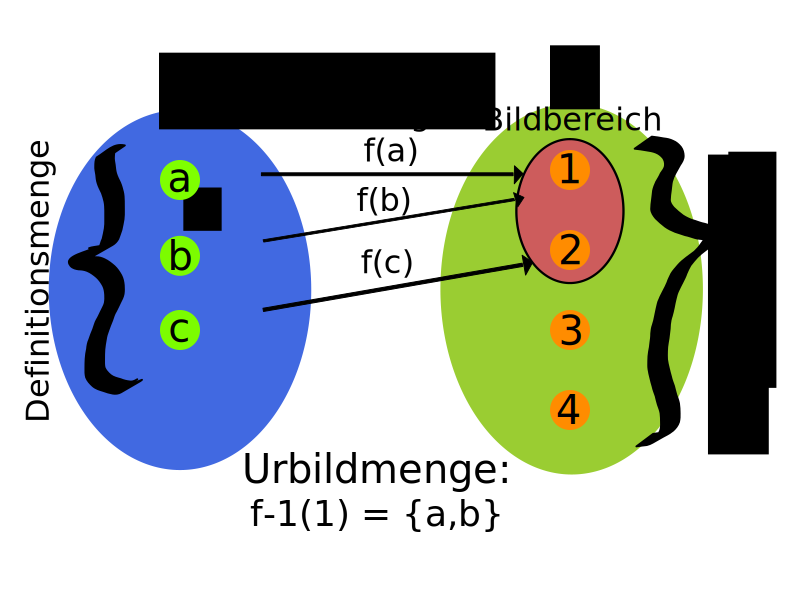
\includegraphics[scale=0.5]{abbildung.pdf}
%%% Local Variables:
%%% mode: latex
%%% TeX-master: "../script"
%%% End:

\paragraph{Hinweis:}
Der Begriff \emph{Wertemenge} kann als Synonym sowohl für die \emph{Zielmenge}
als auch für den \emph{Bildbereich} verwendet werden. In diesem Skript sind
\emph{Zielmenge} und {Wertemenge} identisch, der \emph{Bildbereich} ist somit
eine Teilmenge der \emph{Wertemenge}.
